\documentclass{article}
\usepackage[utf8]{inputenc}
\usepackage{amsmath}
\usepackage{graphicx}
\usepackage[ ]{algorithm2e} 

\title{Document}
\author{Qiujiang Jin}
\date{ }
 
\renewcommand*\contentsname{Content}

\begin{document}
 
\maketitle
 
\tableofcontents
 
\section{Introduction}
 
This is the modeling document for the software that solves the steady-state heat equation in one- and two-dimensions. This document highlights the governing equations, nomenclature, boundary conditions, numerical approximations, algorithms to implement the solver, required memory, verification methodology, input/runtime options, build procedures and example results.

\section{Preliminary}

\subsection*{2.1 Equations}
\addcontentsline{toc}{subsection}{2.1 Equations}
The steady-state heat equation with a constant coefficient in one dimensions is given by:
\[
-k\frac{d^2 T(x)}{dx^2} = q(x)\quad
x \in (0, 1)
\]
Where k is the given constant and it means thermal conductivity, T is the function we want to solve and it means material temperature, and q is the given function and it means the heat source term. There is only one equation. The steady-state heat equation with a constant coefficient in two dimensions is given by:
\[
-k{\nabla}^2{T(x, y)} = q(x, y)\quad
(x, y) \in \Omega = (0, 1)\times(0, 1)
\]
which is equivalent to
\[
-k(\frac{\partial^2 T(x, y)}{\partial x^2} + \frac{\partial^2 T(x, y)}{\partial y^2})= q(x, y)
\]

\subsection*{2.2 Boundary Conditions}
\addcontentsline{toc}{subsection}{2.2 Boundary Conditions}
I choose to use the Dirichlet boundary conditions. So for the one dimensional case it is:
\[
T(0) = \alpha \quad T(1) = \beta
\]
Where $\alpha$ and $\beta$ are 2 given constants. For the second dimensional case it is:
\[
T(x, y)|_{\partial\Omega} = f(x, y)
\]
Where $f(x, y)$ is the given function defined on $\partial\Omega$

\subsection*{2.3 Other Assumptions}
\addcontentsline{toc}{subsection}{2.3 Other Assumptions}
We know the values of $k$ and function $q(x, y)$. We also know the values of $\alpha$, $\beta$ and the boundary function $f(x, y)$. The domain for the one dimensional case is $(0, 1)$ and the mesh sizes are all equal to $h$. The domain for the two dimensional case is $\Omega = (0, 1)\times(0, 1)$ and the mesh sizes are all equal to $h$ for both x-axis and y-axis. My scheme is node-based and I assume a square domain for the 2D case. For the 4th order scheme, I also assume to know the boundary condition of the points outside of the bound so that I can establish the linear system for the points near the boundary.
 
\section{Numerical Methods}

\subsection*{3.1 Finite Difference Methods}
\addcontentsline{toc}{subsection}{3.1 Finite Difference Methods}
Using the Taylor expansion we can derive the finite-difference approximations for the second derivative
in the heat equation. For the one dimensional case, we have 2nd-order finite-difference approximations:
\[
\frac{d^2 T(x)}{dx^2} = \frac{T(x+h) + T(x-h) - 2T(x)}{h^2} - \frac{2h^2}{4!}\frac{d^4 T(x)}{dx^4} + O(h^4)
\]
Denote $x_i = ih$ and $T_i = T(x_i)$, the discrete approximations of the heat equation using these formulations is:
\[
\frac{d^2 T(x_i)}{dx^2} = \frac{T_{i+1} + T_{i-1} - 2T_i}{h^2} - \frac{2h^2}{4!}\frac{d^4 T(x_i)}{dx^4} + O(h^4)
\]
So we have:
\[
-k\frac{T_{i+1} + T_{i-1} - 2T_i}{h^2} = q(x_i)
\]
we have 4th-order finite-difference approximations:
\[
\begin{split}
\frac{d^2 T(x)}{dx^2} &= \frac{- T(x+2h) + 16T(x+h) - 30T(x) + 16T(x-h) - T(x-2h)}{12h^2}\\
                                 &+ \frac{8h^4}{6!}\frac{d^6 T(x)}{dx^6} + O(h^6)
\end{split}
\]
The discrete approximations of the heat equation using these formulations is:
\[
\begin{split}
\frac{d^2 T(x_i)}{dx^2} &= \frac{- T_{i+2} + 16T_{i+1} - 30T_i + 16T_{i-1} - T_{i-2}}{12h^2}\\
                                    &+ \frac{8h^4}{6!}\frac{d^6 T(x_i)}{dx^6} + O(h^6)
\end{split}
\]
So we have:
\[
-k\frac{- T_{i+2} + 16T_{i+1} - 30T_i + 16T_{i-1} - T_{i-2}}{12h^2} = q(x_i)
\]\\ \\
And similarly, we can derive  the 2nd-order finite-difference approximations for the second dimensional case:
\[
\begin{split}
{\nabla}^2{T(x, y)} &= \frac{T(x+h, y) + T(x-h, y) - 2T(x, y)}{h^2} + \frac{T(x, y+h) + T(x, y-h) - 2T(x, y)}{h^2}\\ 
                             &- \frac{2h^2}{4!}(\frac{\partial^4 T(x, y)}{\partial x^4} + \frac{\partial^4 T(x, y)}{\partial y^4}) + O(h^4)
\end{split}
\]
Denote $x_i = ih$, $y_j = jh$ and $T_{i, j} = T(x_i, y_j)$, the discrete approximations of the heat equation using these formulations is:
\[
\begin{split}
{\nabla}^2{T(x_i, y_j)} &= \frac{T_{i+1,j} + T_{i-1,j} - 2T_{i, j}}{h^2} + \frac{T_{i, j+1} + T_{i, j-1} - 2T_{i, j}}{h^2}\\ 
                             &- \frac{2h^2}{4!}(\frac{\partial^4 T(x_i, y_j)}{\partial x^4} + \frac{\partial^4 T(x_i, y_j)}{\partial y^4}) + O(h^4)
\end{split}
\]
So we have:
\[
-k(\frac{T_{i+1,j} + T_{i-1,j} - 2T_{i, j}}{h^2} + \frac{T_{i, j+1} + T_{i, j-1} - 2T_{i, j}}{h^2}) = q(x_i, y_j)
\]\\ \\
we have 4th-order finite-difference approximations:
\[
\begin{split}
{\nabla}^2{T(x, y)}  &= \frac{- T(x+2h, y) + 16T(x+h, y) - 30T(x, y) + 16T(x-h, y) - T(x-2h, y)}{12h^2}\\
                              &+ \frac{- T(x, y+2h) + 16T(x, y+h) - 30T(x, y) + 16T(x, y-h) - T(x, y-2h)}{12h^2}\\
                              &+ \frac{8h^4}{6!}(\frac{\partial^6 T(x, y)}{\partial x^6} + \frac{\partial^6 T(x, y)}{\partial y^6})  + O(h^6)
\end{split}
\]
The discrete approximations of the heat equation using these formulations is:
\[
\begin{split}
{\nabla}^2{T(x_i, y_j)} &= \frac{- T_{i+2, j} + 16T_{i+1, j} - 30T_{i, j} + 16T_{i-1, j} - T_{i-2, j}}{12h^2}\\
                                   &+ \frac{- T_{i, j+2} + 16T_{i, j+1} - 30T_{i, j} + 16T_{i, j-1} - T_{i, j-2}}{12h^2}\\
                                   &+ \frac{8h^4}{6!}(\frac{\partial^6 T(x_i, y_j)}{\partial x^6} + \frac{\partial^6 T(x_i, y_j)}{\partial y^6})  + O(h^6)
\end{split}
\]
So we have:
\[
\begin{split}
&-k(\frac{- T_{i+2, j} + 16T_{i+1, j} - 30T_{i, j} + 16T_{i-1, j} - T_{i-2, j}}{12h^2}\\
&+ \frac{- T_{i, j+2} + 16T_{i, j+1} - 30T_{i, j} + 16T_{i, j-1} - T_{i, j-2}}{12h^2})= q(x_i, y_j)
\end{split}
\]

\subsection*{3.2 Figures of Discretized Meshes}
\addcontentsline{toc}{subsection}{3.2 Figures of Discretized Meshes}
Here is the representative figures of 2D discretized meshes with domain $\Omega = (0, 1)\times(0, 1)$ and mesh size $h = 0.1$ for both axis. My scheme is node-based. The domain is meshed in squares.
\begin{figure}[h]
  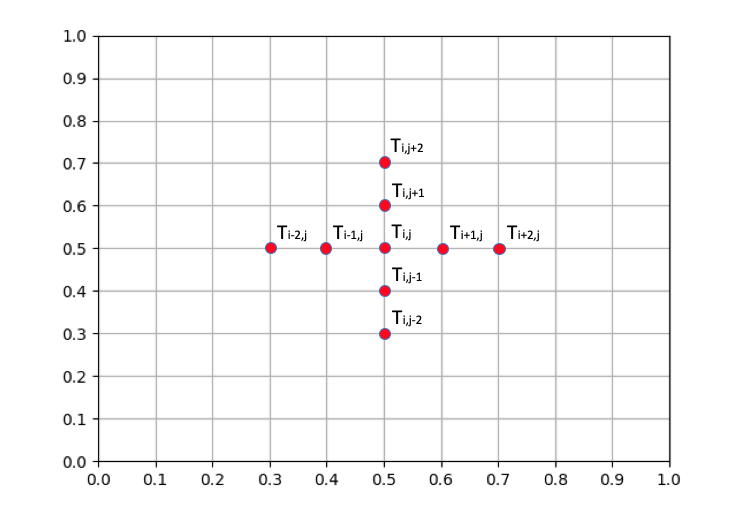
\includegraphics[width=\linewidth]{figure_2}
  \caption{figures of 2D discretized meshes}
\end{figure}

Here is the representative figures of 1D discretized meshes with domain $(0, 1)$ and mesh size $h = 0.1$

\newpage

\begin{figure}[h]
  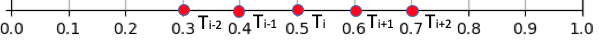
\includegraphics[width=\linewidth]{figure_1}
  \caption{figures of 1D discretized meshes}
\end{figure}

\subsection*{3.3 Linear Systems}
\addcontentsline{toc}{subsection}{3.3 Linear Systems}
First consider the 2nd-order finite-difference schemes
For the one dimensional case, consider $N = \frac{1}{h}$. Then $x_0 = 0$ and $x_N = 1$. We want to solve $T_i$ for $1 \leq i \leq N-1$. And $T_0 = T(x_0) = T(0) = \alpha$ and $T_N = T(x_N) = T(1) = \beta$. So the linear system is:
$$
\left\{
\begin{aligned}
& i = 1 & -k\frac{T_{0} + T_{2} - 2T_1}{h^2}  \quad \quad  \quad \quad  \quad \quad  \quad \quad  \quad \quad & = q(x_1) \\
& i = 2 & -k\frac{T_{1} + T_{3} - 2T_2}{h^2}   \quad \quad  \quad \quad  \quad \quad  \quad \quad & = q(x_2) \\
& i = 3 & -k\frac{T_{2} + T_{4} - 2T_3}{h^2}   \quad \quad  \quad \quad  \quad \quad & = q(x_3) \\
& ......\\
& i = N-1 & -k\frac{T_{N-2} + T_{N} - 2T_{N-1}}{h^2}  & = q(x_{N-1})
\end{aligned}
\right.
$$
Matrix Form $A_1t_1 = b_1$ with $A_1 \in R^{N-1\times N-1}$ and $t_1, b_1 \in R^{N-1}$
\[
A_1 = 
\begin{bmatrix}
    2  & -1 &     &     &  \\
    -1 & 2  & -1 &     & \\
        & -1 &  2 & -1 & \\
        &     & ... &     & \\
        &     &     & -1 & 2  
\end{bmatrix}
\quad t_1 =
\begin{bmatrix}
    T_1\\
    T_2\\
    T_3\\
     ...\\
     T_{N-1}
\end{bmatrix}
\quad b_1 =
\begin{bmatrix}
    \frac{h^2}{k}q(x_1) + \alpha\\
    \frac{h^2}{k}q(x_2) \\
    \frac{h^2}{k}q(x_3)\\
     ...\\
     \frac{h^2}{k}q(x_{N-1}) + \beta
\end{bmatrix}
\]
the number of non-zero entries on an interior row of the matrix $A_1$ is $3$\\ \\
For the second dimensional case, consider $N = \frac{1}{h}$. Then $x_0 = y_0 = 0$ and $x_N = y_N = 1$. We want to solve $T_{i, j}$ for $1 \leq i,j \leq N-1$. And $T_{0, j} = f(0, y_j)$,  $T_{N, j} = f(1, y_j)$ for $0 \leq j \leq N$ and $T_{i, 0} = f(x_i, 0)$, $T_{i, N} = f(x_i, 1)$ for $0 \leq i \leq N$. So the linear system is:
\begin{equation}
-k\frac{T_{i+1,j} + T_{i-1,j} + T_{i, j+1} + T_{i, j-1} - 4T_{i, j}}{h^2} = q(x_i, y_j) \quad 1 \leq i,j \leq N-1
\end{equation}
Matrix Form $A_2t_2 = b_2$ with $A_1 \in R^{(N-1)^2 \times (N-1)^2}$ and $t_1, b_1 \in R^{(N-1)^2}$
\[
A_2 = 
\begin{bmatrix}
    B_2  & -I      &         &     &  \\
    -I      & B_2  & -I      &     & \\
            & -I      &  B_2 & -I & \\
            &         &  ...    &     & \\
            &         &         & -I & B_2  
\end{bmatrix}
\quad B_2 =
\begin{bmatrix}
    4  & -1 &     &     &  \\
    -1 & 4  & -1 &     & \\
        & -1 &  4 & -1 & \\
        &     & ... &     & \\
        &     &     & -1 & 4  
\end{bmatrix}
\]
And $I \in R^{N-1 \times N-1}$ is the identity matrix.
\[
t_2 = [T_{1, 1}, ..... , T_{N-1, 1}, T_{1, 2}, ...... , T_{N-1, 2}, ...... ,T_{1, N-1}, ......, T_{N-1, N-1}]^T
\]
\[
b_2 = [\frac{h^2}{k}q_{x_1, y_1} + f(0, y_1) + f(x_1, 0),\quad...,\quad \frac{h^2}{k}q_{x_i, y_1} + f(x_i, 0),\quad...,\quad \frac{h^2}{k}q_{x_{N-1}, y_1} + f(1, y_1) + f(x_{N-1}, 0),
\]
\[
 ...,\quad \frac{h^2}{k}q_{x_i, y_j},\quad...,
\]
\[  
\frac{h^2}{k}q_{x_1, y_{N-1}} + f(0, y_{N-1}) + f(x_1, 1),\quad...,\quad \frac{h^2}{k}q_{x_i, y_{N-1}} + f(x_i, 1),\quad...,\quad \frac{h^2}{k}q_{x_{N-1}, y_{N-1}} + f(1, y_{N-1}) + f(x_{N-1}, 1)]^T
\]
the number of non-zero entries on an interior row of the matrix $A_2$ is $5$\\ \\
Then consider the 4th-order finite-difference schemes
For the one dimensional case, The linear system is:
\[
-k\frac{- T_{i+2} + 16T_{i+1} - 30T_i + 16T_{i-1} - T_{i-2}}{12h^2} = q(x_i) \quad 1 \leq i \leq N-1
\]
Notice that for $i = 1$ and $i = N-1$ we need information of $T_{-1} = \alpha^{*}$ and $T_{N+1} = \beta^{*}$. Matrix Form $A_3t_3 = b_3$ with $A_3 \in R^{N-1\times N-1}$ and $t_3, b_3 \in R^{N-1}$
\[
A_3 = 
\begin{bmatrix}
    30  & -16 &  1    &       &        &       \\
    -16 & 30  & -16 & 1     &        &       \\
       1 & -16 &  30  & -16 & 1     &       \\
          &       &  ...   &   ...  &  ...   &       \\
          &       &   1   & -16  & 30   & -16 \\
          &       &        &    1  &  -16 &  30
\end{bmatrix}
\quad t_3 =
\begin{bmatrix}
    T_1\\
    T_2\\
    T_3\\
     ...\\
     T_{N-2}\\
     T_{N-1}
\end{bmatrix}
\quad b_3 =
\begin{bmatrix}
    \frac{12h^2}{k}q(x_1) + 16\alpha - \alpha^{*}\\
    \frac{12h^2}{k}q(x_2) - \alpha\\
    \frac{12h^2}{k}q(x_3)\\
     ...\\
      \frac{12h^2}{k}q(x_{N-2}) - \beta\\
      \frac{12h^2}{k}q(x_{N-1}) + 16\beta - \beta^{*}
\end{bmatrix}
\]
the number of non-zero entries on an interior row of the matrix $A_3$ is $5$\\ \\
For the second dimensional case, the linear system is:
\[
-k\frac{- T_{i+2, j} - T_{i-2, j} - T_{i, j+2} - T_{i, j-2} + 16T_{i+1, j} + 16T_{i-1, j} + 16T_{i, j+1} + 16T_{i, j-1} - 60T_{i, j}}{12h^2} = q(x_i, y_j)
\]
\[
1 \leq i, j \leq N-1
\]
Notice that for the point next to the boundary we need information $T_{-1, j} = f^{*}(x_{-1}, y_j)$ and $T_{N+1, j} = f^{*}(x_{N+1}, y_j)$ for $-1 \leq j \leq N+1$ and $T_{i, -1} = f^{*}(x_i, y_{-1})$ and $T_{i, N+1} = f^{*}(x_i, y_{N+1})$ for $-1 \leq i \leq N+1$. Matrix Form $A_4t_4 = b_4$ with $A_4 \in R^{(N-1)^2 \times (N-1)^2}$ and $t_4, b_4 \in R^{(N-1)^2}$
\[
A_4 = 
\begin{bmatrix}
    R    &  Q   &  P    &        &      &     \\
    Q    &  R   &  Q   &  P    &      &     \\
    P     &  Q  &  R   &  Q    &  P  &      \\
           &       &  ...   &   ...  &  ...  &      \\
           &       &   P   &  Q   &  R  &  Q  \\
           &       &        &   P   &  Q  &  R
\end{bmatrix}
\]
\[
P =
\begin{bmatrix}
    1  &  &     &     &  \\
        &  1  &  &     & \\
        &    &  1 &   & \\
        &     & ... &     & \\
        &  &  &  1&   \\
        &     &     &   &  1
\end{bmatrix}
\quad Q =
\begin{bmatrix}
  -16 &  &     &     &  \\
        & -16  &  &     & \\
        &    &  -16 &   & \\
        &     & ... &     & \\
        &  &  &  -16&   \\
        &     &     &   & -16  
\end{bmatrix}
\]
\[
R =
\begin{bmatrix}
    60  & -16 &   1   &        &       &     \\
    -16 & 60  & -16 & 1     &        &     \\
       1 & -16 &  60  & -16 & 1     &      \\
          &       &  ...   &   ...  &  ...   &      \\
          &       &   1   & -16  & 60   & -16 \\
          &       &        &    1  &  -16 & 60
\end{bmatrix}
\]
Where $I \in R^{N-1 \times N-1}$ is the indentity matrix.
\[
t_4 = [T_{1, 1}, ..... , T_{N-1, 1}, T_{1, 2}, ...... , T_{N-1, 2}, ...... ,T_{1, N-1}, ......, T_{N-1, N-1}]^T
\]
\[
b_4 = [
\]
\[
\frac{12h^2}{k}q_{x_1, y_1} + 16f(0, y_1) + 16f(x_1, 0) - f^{*}(x_{-1}, y_1) - f^{*}(x_1, y_{-1}),\frac{12h^2}{k}q_{x_2, y_1} + 16f(x_2, 0) - f^(0, y_1) - f^{*}(x_2, y_{-1}), 
\]
\[
 ...,\quad \frac{12h^2}{k}q_{x_i, y_1} + 16f(x_i, 0) - f^{*}(x_i, y_{-1}),\quad...,
\]
\[
\frac{12h^2}{k}q_{x_{N-2}, y_1} + 16f(x_{N-2}, 0) - f(1, y_1) - f^{*}(x_{N-2}, y_{-1}),
\]
\[
\frac{12h^2}{k}q_{x_{N-1}, y_1} + 16f(1, y_1) + 16f(x_{N-1}, 0) - f^{*}(x_{N+1}, y_1) - f^{*}(x_{N-1}, y_{-1}),
\]
\[
\frac{12h^2}{k}q_{x_1, y_2} + 16f(0, y_2) - f^{*}(x_{-1}, y_2) - f(x_1, 0),\frac{12h^2}{k}q_{x_2, y_1} - f(0, y_1) - f(x_2, 0), 
\]
\[
 ...,\quad \frac{12h^2}{k}q_{x_i, y_2} - f(x_i, 0),\quad...,
\]
\[
\frac{12h^2}{k}q_{x_{N-2}, y_2}  - f(1, y_2) - f(x_{N-2}, 0), \frac{12h^2}{k}q_{x_{N-1}, y_2} + 16f(1, y_2) - f^{*}(x_{N+1}, y_2) - f(x_{N-1}, 0),
\]
\[
...,\quad \frac{12h^2}{k}q_{x_1, y_j} + 16f(0, y_j) - f^{*}(x_{-1}, y_j),\frac{12h^2}{k}q_{x_2, y_j} - f(0, y_j),
\]
\[
 ...,\quad \frac{12h^2}{k}q_{x_i, y_j},\quad...,
\]
\[
\frac{12h^2}{k}q_{x_{N-2}, y_j}  - f(1, y_j), \frac{12h^2}{k}q_{x_{N-1}, y_j} + 16f(1, y_j) - f^{*}(x_{N+1}, y_j),\quad...,
\]
\[
\frac{12h^2}{k}q_{x_1, y_{N-2}} + 16f(0, y_{N-2}) - f^{*}(x_{-1}, y_{N-2}) - f(x_1, 1),\frac{12h^2}{k}q_{x_2, y_{N-2}} - f(0, y_{N-2}) - f(x_2, 1), 
\]
\[
 ...,\quad \frac{12h^2}{k}q_{x_i, y_{N-2}} - f(x_i, 0),\quad...,
\]
\[
\frac{12h^2}{k}q_{x_{N-2}, y_{N-2}}  - f(1, y_{N-2}) - f(x_{N-2}, 0), \frac{12h^2}{k}q_{x_{N-1}, y_{N-2}} + 16f(1, y_{N-2}) - f^{*}(x_{N+1}, y_{N-2}) - f(x_{N-1}, 1),
\]
\[
\frac{12h^2}{k}q_{x_1, y_{N-1}} + 16f(0, y_{N-1}) + 16f(x_1, 1) - f^{*}(x_{-1}, y_{N-1}) - f^{*}(x_1, y_{N+1}),
\]
\[
\frac{12h^2}{k}q_{x_2, y_{N-1}} + 16f(x_2, 1) - f(0, y_{N-1}) - f^{*}(x_2, y_{N+1}), 
\]
\[
 ...,\quad \frac{12h^2}{k}q_{x_i, y_{N-1}} + 16f(x_i, 1) - f^{*}(x_i, y_{N+1}),\quad...,
\]
\[
\frac{12h^2}{k}q_{x_{N-2}, y_{N-1}} + 16f(x_{N-2}, 0) - f(1, y_{N-1}) - f^{*}(x_{N-2}, y_{N+1}),
\]
\[
\frac{12h^2}{k}q_{x_{N-1}, y_{N-1}} + 16f(1, y_{N-1}) + 16f(x_{N-1}, 1) - f^{*}(x_{N+1}, y_{N-1}) - f^{*}(x_{N-1}, y_{N+1}),]^T
\]
the number of non-zero entries on an interior row of the matrix $A_4$ is $9$

\subsection*{3.4 Algorithms to Solve Linear Systems}
\addcontentsline{toc}{subsection}{3.4 Algorithms to Solve Linear Systems}
I use 2 simple iterative methods to solve the linear system.\\
First consider the Jacobi method to solve $Ax = b$\\
Suppose $A = D + R$ where $D$ is the diagonal component of $A$ and $R$ is the remainder. The Jacobi method is $x^{k+1} = D^{-1}(b - Rx^{k})$, which is equivalent to:
\[
x_i^{k+1} = \frac{1}{a_{ii}}(b_i - \sum_{j \neq i}a_{ij}x_j^{k}) \quad i = 1, ......, n
\]
The pseudo-code is the following:\\ \\
\begin{algorithm}[H]
\SetAlgoLined
 \textbf{Input}: initial guess $x^0$, diagonal dominant matrix A, right handed vector b, convergence criterion $\epsilon$\\
 \textbf{Output}: solution when convergence is reached\\
 $k = 0$\\
 \While{ $|| b - Ax^{k} || \geq \epsilon$ }{
   \For{$i := 1$ to $n$}{
     $s = 0$\\
       \For{$j := 1$ to $n$}{
           \If{$j \neq i$}{
             $s = s + a_{ij}x_j^k$\\
           }
      }
      $x_i^{k+1} = \frac{1}{a_{ii}}(b_i - s)$\\
   }
   $k = k + 1$\\
 }
 \caption{Jacobi Method}
\end{algorithm}
Then consider the Gauss Seidel method to solve $Ax = b$\\
Suppose $A = L + U$ where $L$ is the diagonal and lower triangular component of $A$ and $U$ is the strictly upper triangular component of $A$. The Gauss Seidel method is $x^{k+1} = L^{-1}(b - Ux^{k})$, which is equivalent to:
\[
x_i^{k+1} = \frac{1}{a_{ii}}(b_i - \sum_{j = 1}^{i-1}a_{ij}x_j^{k+1} -  \sum_{j = i+1}^{n}a_{ij}x_j^{k}) \quad i = 1, ......, n
\]
The pseudo-code is the following:\\ \\
\begin{algorithm}[H]
\SetAlgoLined
 \textbf{Input}: initial guess $x^0$, diagonal dominant matrix A, right handed vector b, convergence criterion $\epsilon$\\
 \textbf{Output}: solution when convergence is reached\\
 $k = 1$\\
 \While{ $|| b - Ax^{k} || \geq \epsilon$ }{
   \For{$i := 1$ to $n$}{
     $s = 0$\\
       \For{$j := 1$ to $i-1$}{
            $s = s + a_{ij}x_j^k$\\
       }
       \For{$j := i+1$ to $n$}{
            $s = s + a_{ij}x_j^{k-1}$\\
       }
       $x_i^{k} = \frac{1}{a_{ii}}(b_i - s)$\\
   }
   $k = k + 1$\\
 }
 \caption{Gauss Seidel Method}
\end{algorithm}

\subsection*{3.5 Required Memory}
\addcontentsline{toc}{subsection}{3.5 Required Memory}
I use sparse matrix in my numerical implementation. So just need to store the position(which is an integer) and the value(which is double-precision float number) of the non-zero elements in the matrix. So the memory of the matrix is just the number of non-zero elements times $12$ Bytes($4$ Bytes for integer and $8$ Bytes for double-precision float number). And for the right hand sided vector each element requires $8$ Bytes.\\ \\
For the one dimensional problem, the 2nd-order schemes requires $(3N\times12 + N\times8) = 44N$ Bytes. the 4th-order schemes requires $(5N\times12 + N\times8) = 68N$ Bytes.\\ \\
For the two dimensional problem, the 2nd-order schemes requires $(5N^2\times12 + N^2\times8) = 68N^2$ Bytes. the 4th-order schemes requires $(9N^2\times12 + N^2\times8) = 116N^2$ Bytes.

\section{Implementation}

\subsection*{4.1 Build Procedures}
\addcontentsline{toc}{subsection}{4.1 Build Procedures}
Here is how to build the code\\ \\
\$ autoreconf -i\\ \\
\$ module load hdf5\\ \\
\$ module load petsc/3.9-uni\\ \\
\$ export PKGPATH=/work/00161/karl/stampede2/public\\ \\
\$ ./configure \--\--with-masa=\$PKGPATH/masa-gnu7-0.50 \\
\--\--with-grvy=\$PKGPATH/grvy-gnu7-0.34 \--\--with-hdf5=\$TACC\_HDF5\_DIR\\ \\
Then you can $make$ or $make$ $check$ and run the code: $./solver$ $input.dat$

\subsection*{4.2 Input Options}
\addcontentsline{toc}{subsection}{4.2 Input Options}
Here is the various input options relevant for your code
\begin{enumerate}
	\item dimension\\
		dimension is either 1 or 2
	\item xmin\\
		minimal location on the x-axis
	\item xmax\\
		maximal location on the x-axis
	\item ymin\\
		minimal location on the y-axis
	\item ymax\\
		maximal location on the y-axis
	\item nx\\
		number of mesh points on the x-axis
	\item ny\\
		number of mesh points on the y-axis
	\item fd\_method\\
		finite difference scheme is either 2 or 4
	\item iter\_method\\
		iteration method is either Jacobi or Gauss-Seidel
	\item verify\_mode\\
		verification mode is either 0 or 1. 0 means to use the verification and 1 means not to use the verification
	\item output\_mode\\
		output mode is either 0 or 1. 0 means standard output mode and 1 means debug output mode
	\item k\\
		k is the thermal conductivity
	\item eps\\
		This is the error tolerance of the iterative solver
	\item max\_iter\\
		This is the maximal number of solver iterations
	\item output\_file\\
		This is the name of the file containing numerical solutions generated by the solver
	\item masa\_file\\
		This is the name of the file containing analytical solutions generated by the masa
\end{enumerate}
Notice that for convenience it is required that xmin $<$ xmax, ymin $<$ ymax, xmax $-$ xmin = ymax $-$ ymin, nx = ny. If you give the wrong inputs or inputs that don't obey the requirements, the program will give the error information and exit.

\subsection*{4.3 Verification Procedures}
\addcontentsline{toc}{subsection}{4.3 Verification Procedures}
Make sure that verification mode is 0. Then after building the code, $make$ then $make$ $check$ to run the regression test. Then give the command $./solver$ $input.dat$ to run the code in verification mode. Here is the example of the standard output of verification mode.
\newpage
\begin{figure}[h!]
  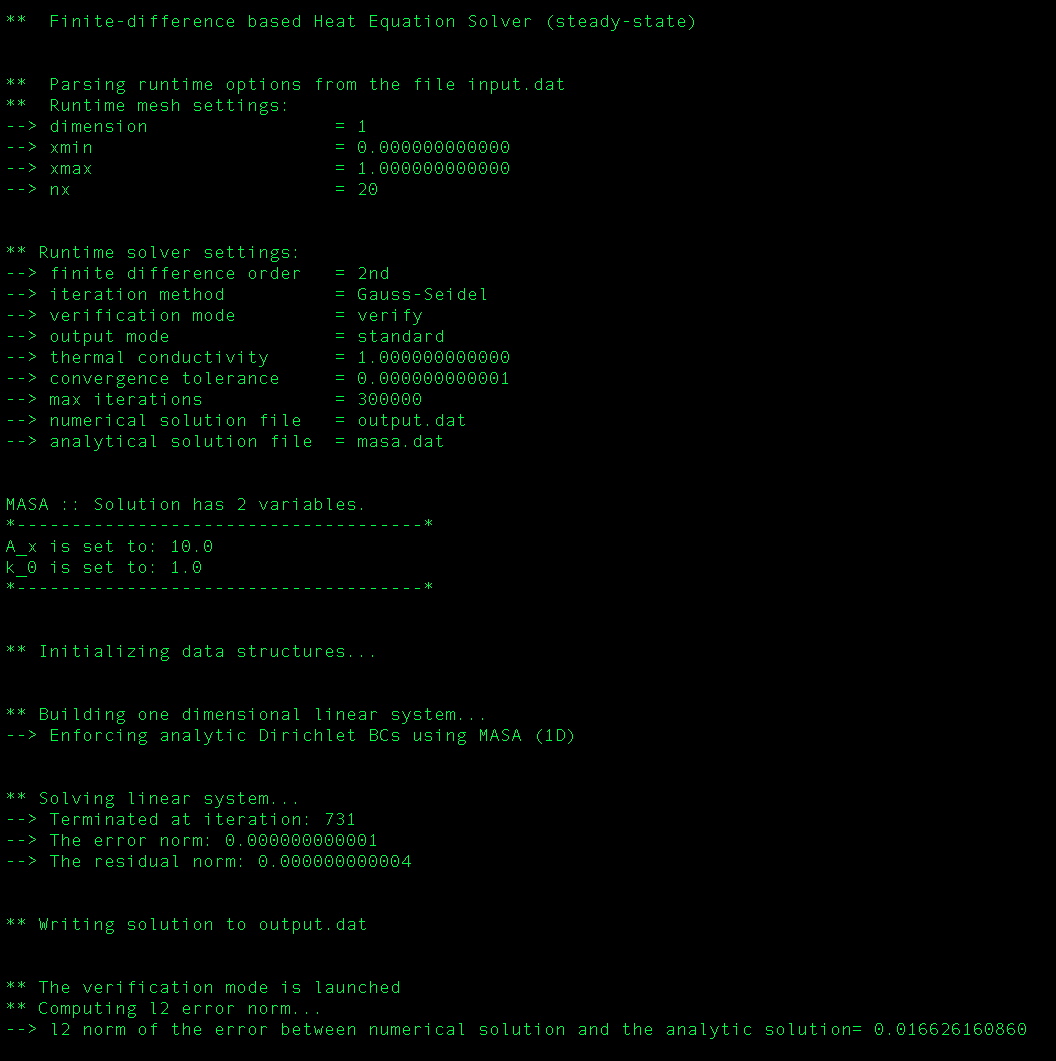
\includegraphics[width=\linewidth]{figure_3}
  \caption{example of the standard output of verification mode}
\end{figure}

\section{Inprovement}

\subsection*{6.1 Code Coverage}
\addcontentsline{toc}{subsection}{6.1 Code Coverage}
Figure 4 is the result of the code coverage:
\begin{figure}[h!]
  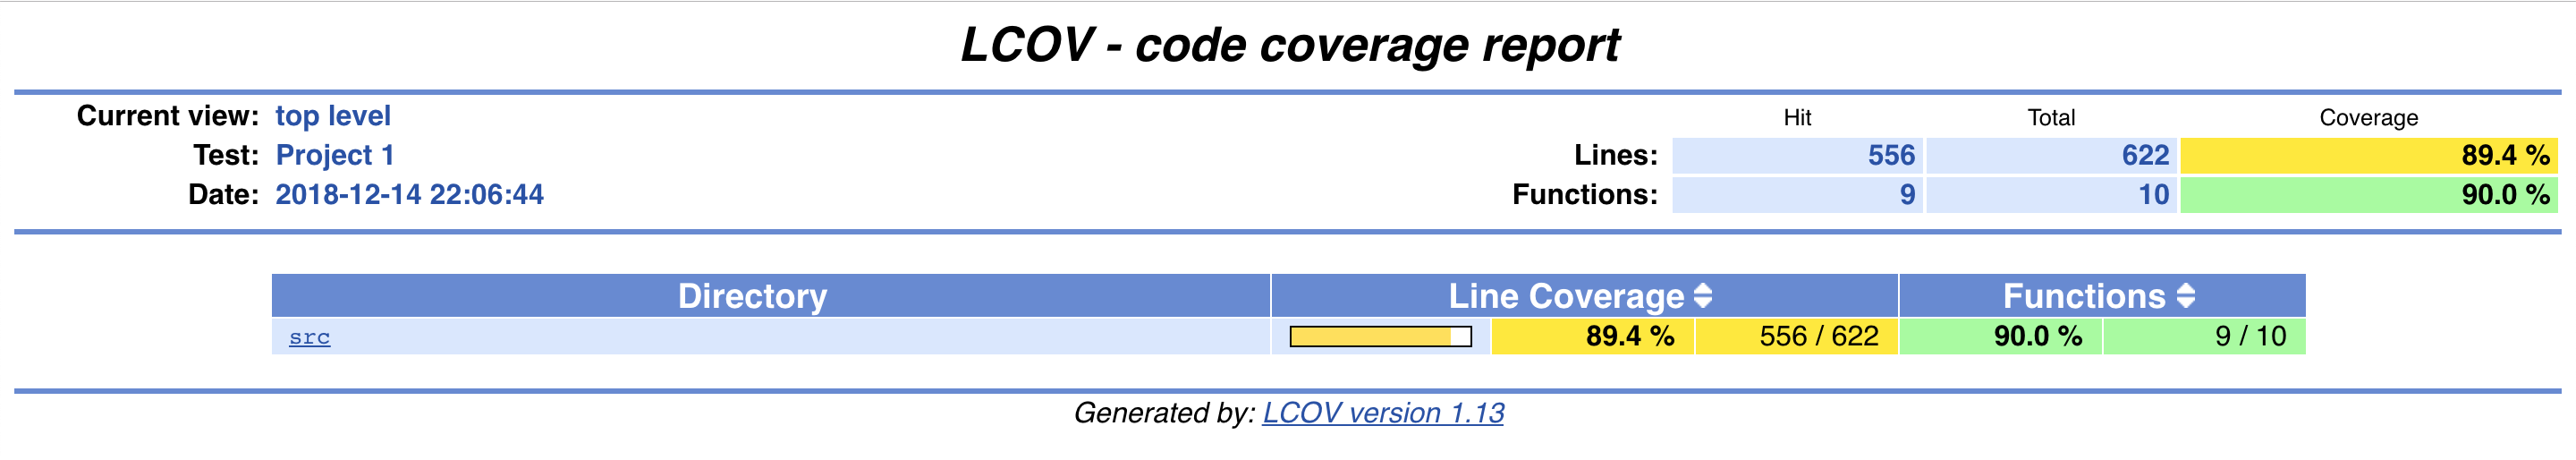
\includegraphics[width=15cm]{figure_13}
  \caption{Report of Code Coverage}
\end{figure}

\subsection*{6.2 HDF5}
\addcontentsline{toc}{subsection}{6.2 HDF5}
I add HDF5 and improve the regression test.

\subsection*{6.3 PETSc}
\addcontentsline{toc}{subsection}{6.3 PETSc}
I add PETSc and the runtime is reduced for smaller mesh size. You can see the results in figure 12 and figure 13.

\section{Results}

\subsection*{6.1 Verification Exercise}
\addcontentsline{toc}{subsection}{6.1 Verification Exercise}
Figure 5, 6 and 7 are the figures of the functions given by analytical and numerical solutions. You can compare them and see that the numerical solutions are very closed to the analytical solutions. Figure 8, 9 and 10 are the plottings of the resulting error norms from the 2nd and 4th order uniform refinement studies. The slope of 2nd order scheme is approximately -2 and the slope of 4th order scheme is approximately -4. They are closed the expected asymptotic convergence rates. I use Matlab to plot the figures of the results.


\begin{figure}[h!]
  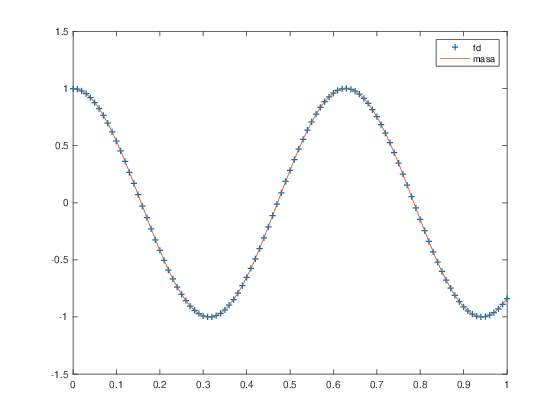
\includegraphics[width=8cm]{figure_4}
  \caption{1D heat equation finite difference solution compared with analytical solution given by MASA}
\end{figure}

\begin{figure}[h!]
  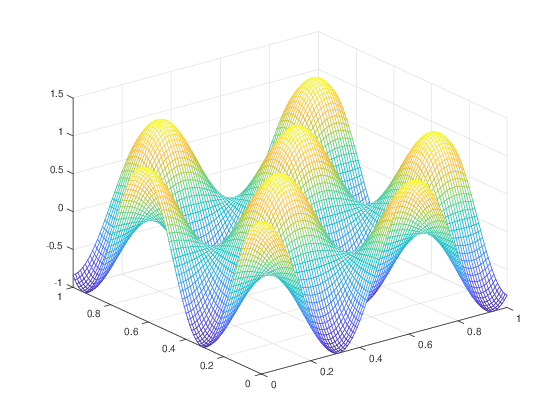
\includegraphics[width=8cm]{figure_5}
  \caption{2D heat equation finite difference solution}
\end{figure}

\begin{figure}[h!]
  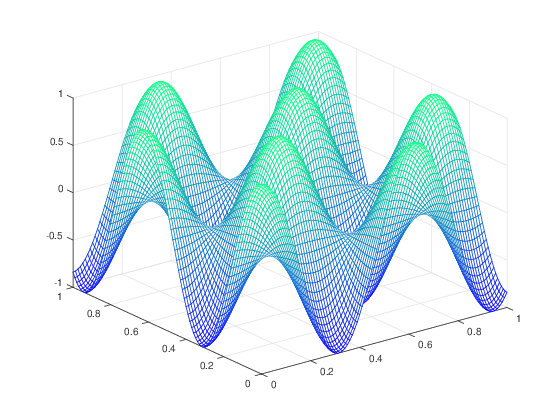
\includegraphics[width=8cm]{figure_6}
  \caption{2D heat equation analytical solution given by MASA}
\end{figure}

\begin{figure}[h!]
  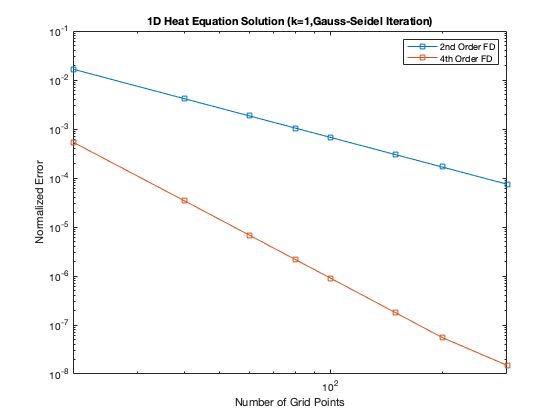
\includegraphics[width=8cm]{figure_7}
  \caption{The slope of 2nd order FD is -2.07 and the slope of 4th order FD is -3.98}
\end{figure}

\begin{figure}[h!]
  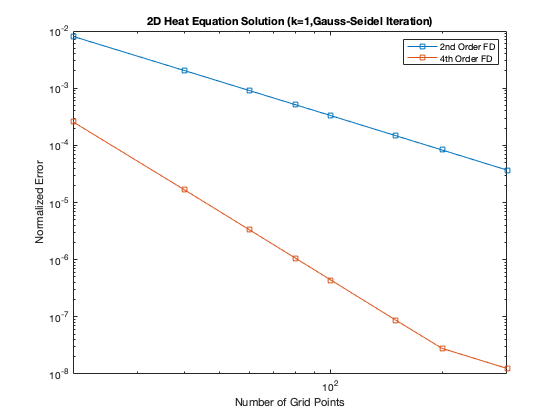
\includegraphics[width=8cm]{figure_8}
  \caption{The slope of 2nd order FD is -2.03 and the slope of 4th order FD is -4.05}
\end{figure}

\begin{figure}[h!]
  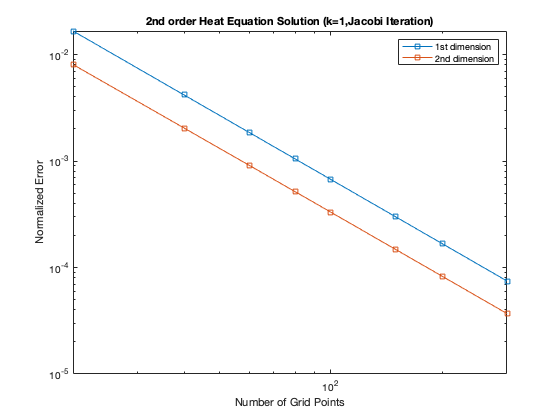
\includegraphics[width=8cm]{figure_9}
  \caption{The slope of 1st dimension is -2.04 and the slope of 2nd dimension is -2.03}
\end{figure}

\subsection*{6.2 Runtime Performance}
\addcontentsline{toc}{subsection}{6.2 Runtime Performance}
Figure 11 is the figure presenting runtime performance measurements of my application. The total runtime is split into 5 parts: input, initialize, build linear system, solve linear system and output. Figure 12 and 13 are comparison of runtime between Jacobi, Gauss-Seidel and PETSc for 1 or 2 dimension and 2nd order scheme.

\begin{figure}
  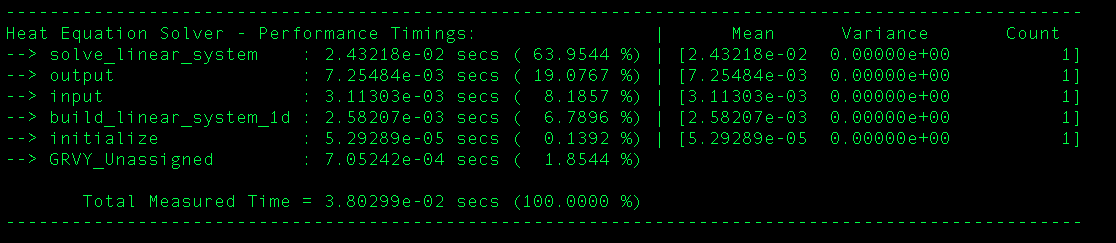
\includegraphics[width=\linewidth]{figure_10}
  \caption{Runtime Performance Measurements}
\end{figure}

\begin{figure}
  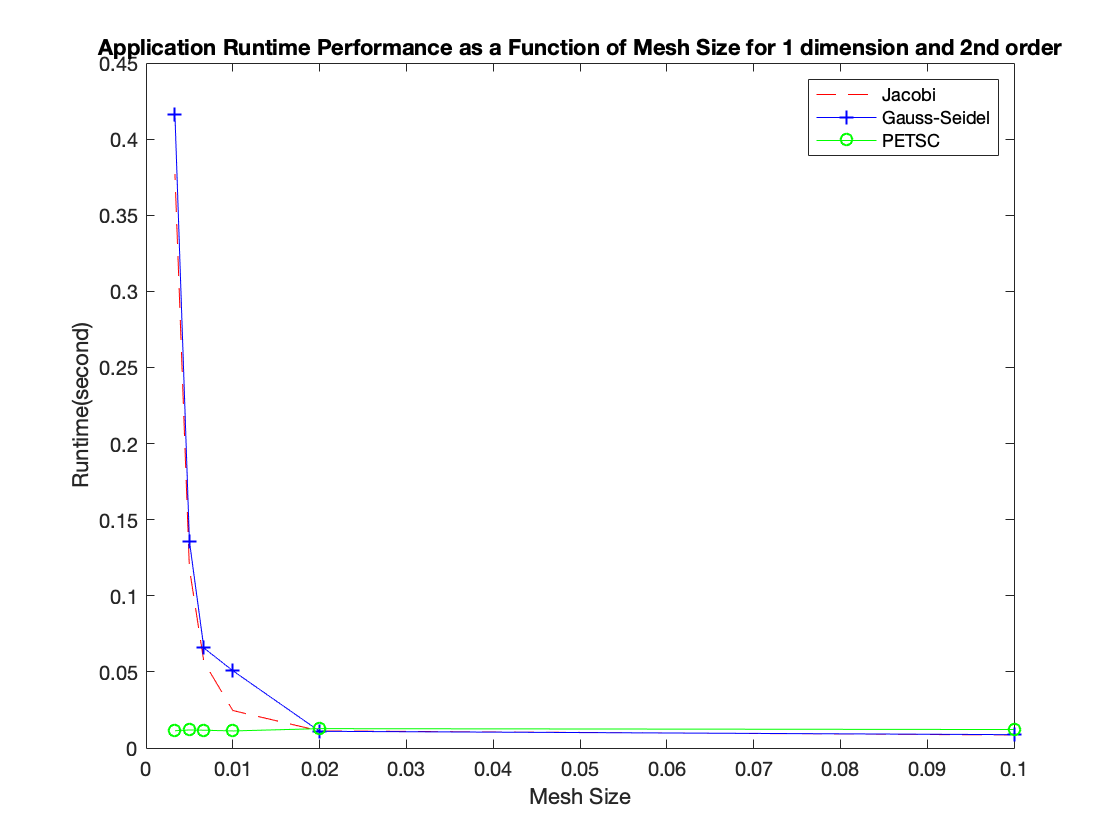
\includegraphics[width=\linewidth]{figure_11}
  \caption{Comparison of Runtime Performance Measurements between different methods}
\end{figure}

\begin{figure}
  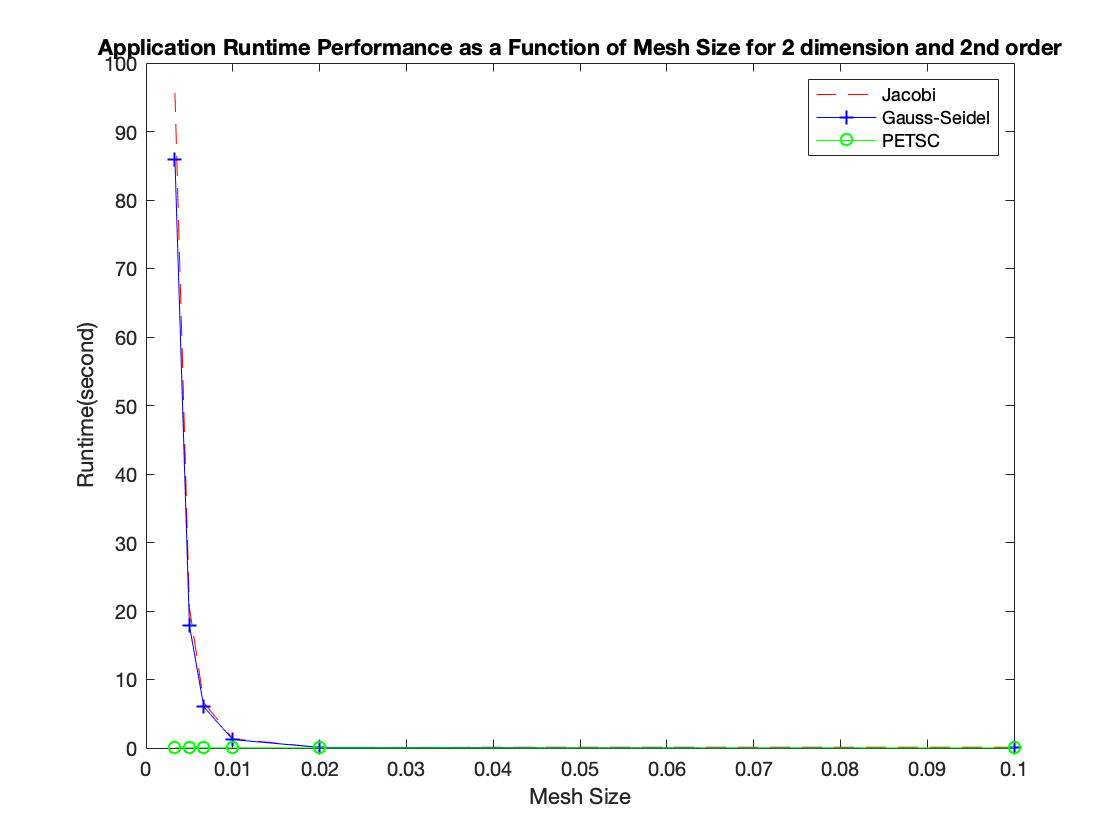
\includegraphics[width=\linewidth]{figure_12}
  \caption{Comparison of Runtime Performance Measurements between different methods}
\end{figure}

\end{document}